\section{Blockschaltbild und Automatengraph}

Zunächst wird ein Blockschaltbild der Schaltung gezeichnet. Das Blockschaltbild wird in \autoref{fig:A1_Block} gezeigt. Die Zustandsrückführung auf das Übergangsschaltnetz ist gestrichelt eingezeichnet, da diese in dieser konkreten Implementierung nicht benötigt wird, weil die Zustandübergänge nur von den Zuständen der Eingangsignal abhängen.

\begin{figure}[H]
    \begin{center}
        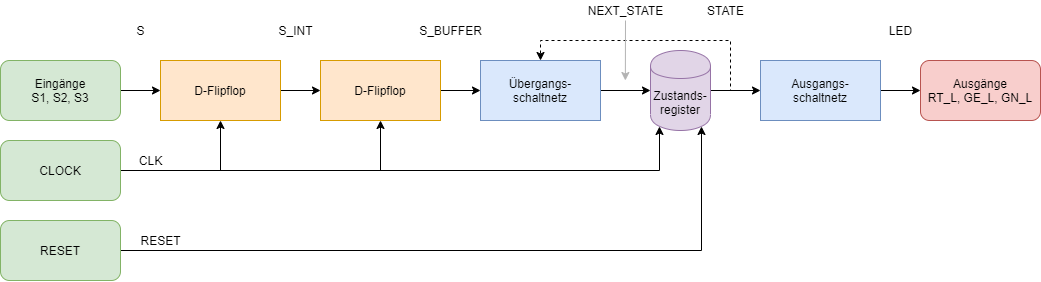
\includegraphics[width=0.9\textwidth]{img/Blockschalt1.png}
        \caption{Blockschaltbild}
        \label{fig:A1_Block}
    \end{center}
\end{figure}


\begin{figure}[H]
    \begin{center}
        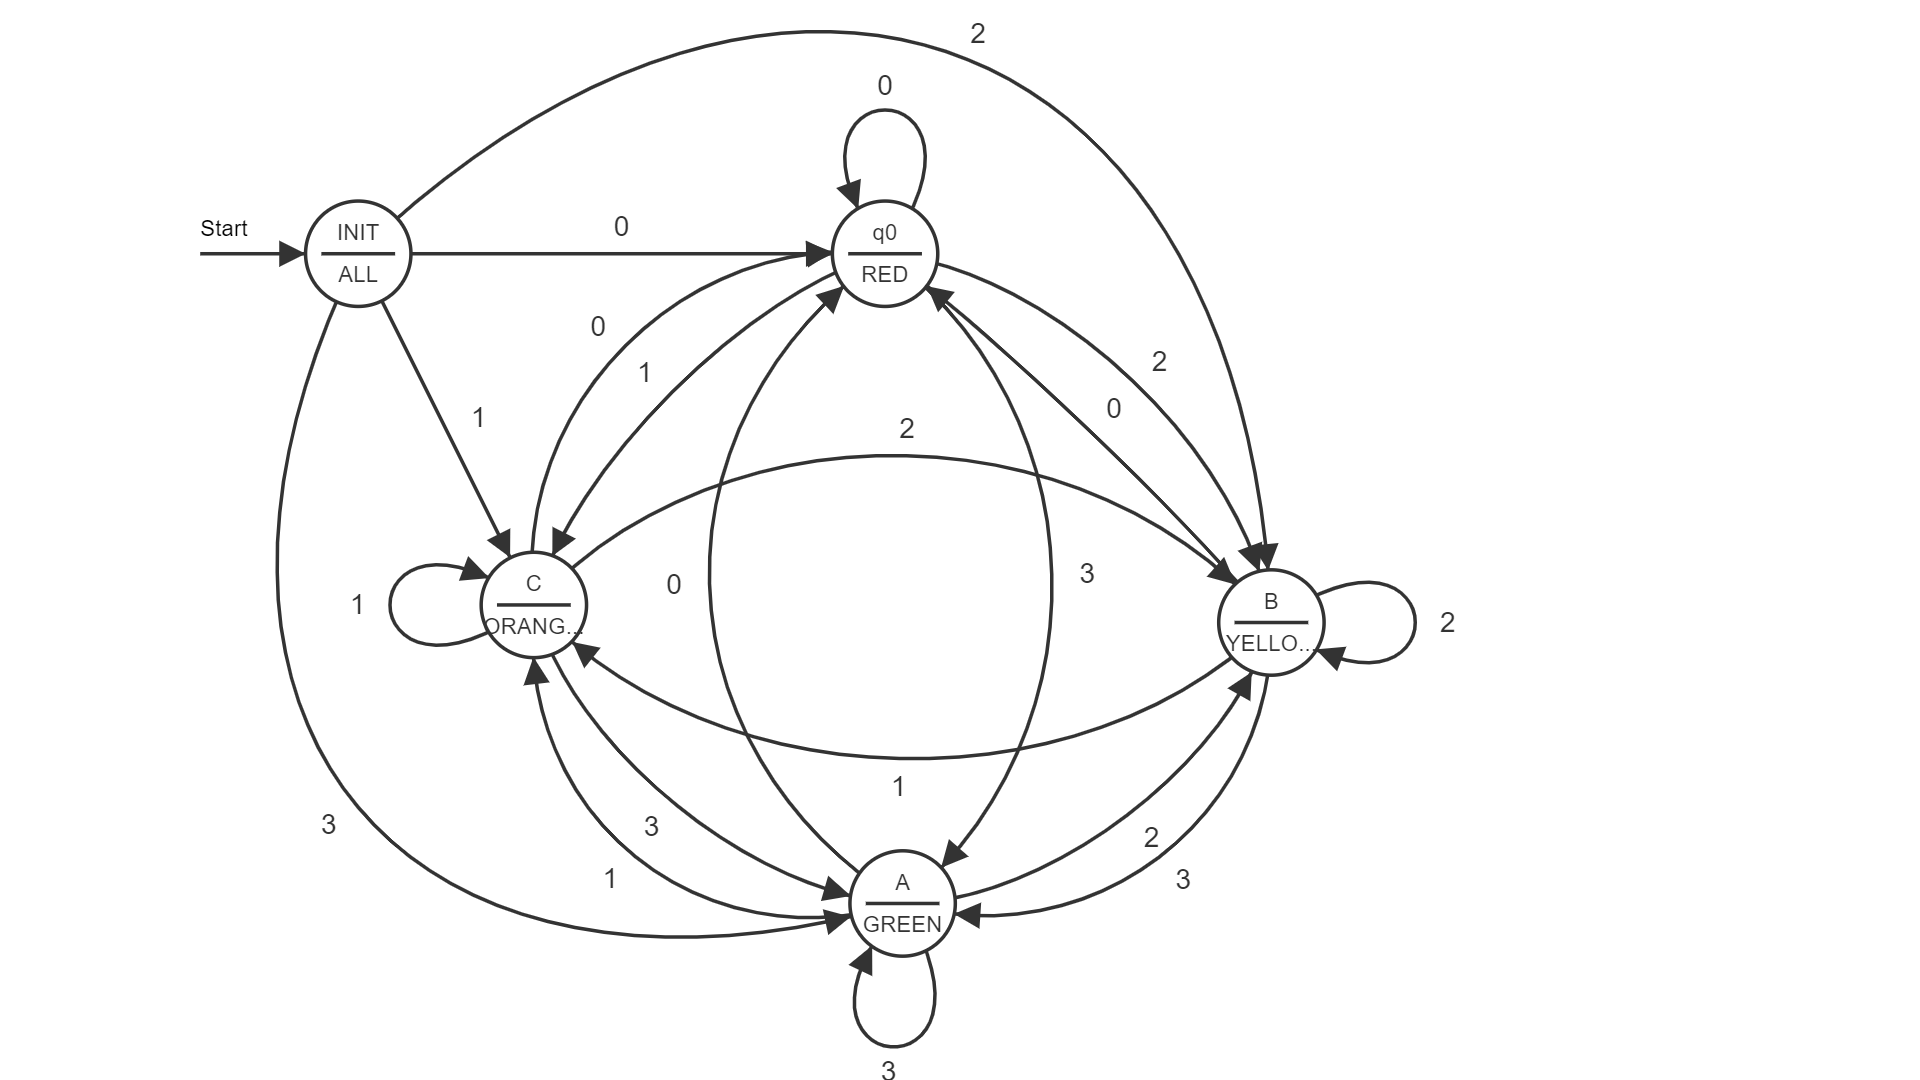
\includegraphics[width=0.8\textwidth]{img/test (2).png}
        \caption{Automatengraph}
        \label{fig:A1_Auto}
    \end{center}
\end{figure}

Das Eingangstupel besteht aus dem Signal der Pumpen-Sensoren. 
%Der Übersichtlichkeit halber wurde auf dem Graph nur modelliert, dass eine Pumpe ausfallen oder wieder funktionieren kann. Der Automat kann Zustände auch überspringen, wenn z.B. zwei Pumpen gleichzeitig ausfallen, dies wurde zwecks Übersichtlichkeit nicht eingezeichnet.
 
Tupel des Automaten:
Zustände:
\[Q =\{Init, A, B, C, D\}  \]
\[mit \ q_0 = Init \]\\
Eingabealphabet:
\[\Sigma =\{0,1,2,3\} \]\\
Ausgabealphabet:
\[\Omega = \{GN\_L, GE\_L, RT\_L\} \]\\
Ausgabefunktion:
\[\lambda = \lambda  : Q \Rightarrow \Omega: \]
\[  \lambda:GN\_L \Rightarrow \Sigma <= 3 \]
\[  \lambda:GE\_L \Rightarrow 0 < \Sigma <= 2  \]
\[  \lambda:RT\_L \Rightarrow  \Sigma <= 1  \]\\


 \begin{table}[H]
    \centering
    \begin{tabular}{|c|c|c|c|c|c|c|}\hline
    \tbf{$\delta$ (Übergang) $\searrow$} & \tbf{$\Sigma= 0$} & \tbf{$\Sigma= 1$}  & \tbf{$\Sigma= 2$} & \tbf{$\Sigma= 3$} & \tbf{$\Delta$ (Ausgabe)} \\ \hline
    $q_0$ = Init    & D     & C     & B     & A     & GN\_L, GE\_L, RT\_L   \\
    A       & D     & C     & B     & A     & GN\_L                 \\ 
    B       & D     & C     & B     & A     & GE\_L                 \\ 
    C       & D     & C     & B     & A     & GE\_L + RT\_L         \\ 
    D       & D     & C     & B     & A     & RT\_L                 \\ \hline
    \end{tabular} 
    \caption{Automatentafel}
\end{table}

